\documentclass[aspectratio=169,12pt]{beamer}
\usetheme{Madrid}
\usecolortheme{dolphin}
\usefonttheme{professionalfonts}
\setbeamertemplate{navigation symbols}{}
\setbeamertemplate{footline}{}

\usepackage[T1]{fontenc}
\usepackage[utf8]{inputenc}
\usepackage{graphicx}
\usepackage{amsmath,amssymb}
\usepackage{hyperref}
\usepackage{siunitx}
\usepackage{physics}
\usepackage{tikz}
\usetikzlibrary{angles,quotes}

\title[Nombres Complexes]{Introduction aux Nombres Complexes}
\author{JAMOTTE Maxime, SCHOONEN Cédric}
\institute{Digital Learning Hub}
\date{}

\begin{document}

\begin{frame}
  \titlepage
\end{frame}

\begin{frame}{Table des matières}
  \tableofcontents
\end{frame}

\section{Motivation}

\begin{frame}{Problème: racine de nombres négatifs}
  Dans l'ensemble des nombres réels $\mathbb{R}$, la racine carrée de nombres négatifs n'existe pas:
  \[
    \sqrt{-1} \quad \text{n'a pas de solution dans } \mathbb{R}
  \]
  
  \bigskip
  \textbf{Solution:} On introduit un nouveau nombre $i$ tel que:
  \[
    i^2 = -1 \qquad \text{ou} \qquad i = \sqrt{-1}
  \]
\end{frame}

\begin{frame}{Construction des nombres complexes}
  À partir de $i$, on peut construire de nouveaux nombres:
  
  \bigskip
  On peut multiplier $i$ par un réel:
  \[
    y \cdot i \qquad \text{avec } y \in \mathbb{R}
  \]
  
  \bigskip
  On peut additionner avec un autre réel:
  \[
    x + yi \qquad \text{avec } x, y \in \mathbb{R}
  \]
  
  \bigskip
  Ceci est la \textbf{forme générale d'un nombre complexe}.
\end{frame}

\begin{frame}{Trois représentations}
  
  \bigskip
  \textbf{Forme cartésienne:}
  \[
    z = x + yi
  \]
  
  \textbf{Forme vectorielle:}
  \[
    z = \begin{pmatrix} x \\ y \end{pmatrix}
  \]
  
  \textbf{Forme polaire:}
  \[
    z = \rho e^{i\theta}
  \]
\end{frame}

\section{Représentation cartésienne/vectorielle}

\begin{frame}{Représentation cartésienne/vectorielle}
  
  %$z = x + yi$ avec $x$ la partie réelle et $y$ la partie imaginaire.
  
  \bigskip
  \begin{center}
  \begin{tikzpicture}[scale=1.8]
    \draw[->] (-0.5,0) -- (3.5,0) node[right] {Re};
    \draw[->] (0,-0.5) -- (0,2.5) node[above] {Im};
    \draw[->,thick,blue] (0,0) -- (2.5,1.5) node[midway,above left] {$z$};
    \draw[dashed] (2.5,0) node[below] {$x$} -- (2.5,1.5);
    \draw[dashed] (0,1.5) node[left] {$y$} -- (2.5,1.5);
    \filldraw[blue] (2.5,1.5) circle (2pt) node[above right] {$x + yi$};
  \end{tikzpicture}
  \end{center}
\end{frame}

\begin{frame}{Addition et soustraction}
  %L'addition se fait composante par composante:
  \[
    (x_1 + y_1 i) + (x_2 + y_2 i) = (x_1+x_2) + (y_1+y_2)i \qquad     \begin{pmatrix} x_1 \\ y_1 \end{pmatrix} + \begin{pmatrix} x_2 \\ y_2 \end{pmatrix} = \begin{pmatrix} x_1 + x_2 \\ y_1 + y_2 \end{pmatrix}
  \]
  
  \begin{center}
  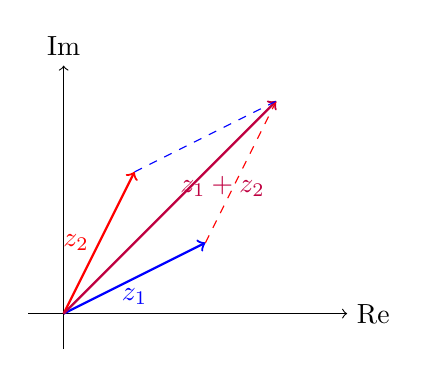
\begin{tikzpicture}[scale=0.9]
    \draw[->] (-0.5,0) -- (4,0) node[right] {Re};
    \draw[->] (0,-0.5) -- (0,3.5) node[above] {Im};
    \draw[->,thick,blue] (0,0) -- (2,1) node[midway,below] {$z_1$};
    \draw[->,thick,red] (0,0) -- (1,2) node[midway,left] {$z_2$};
    \draw[->,thick,purple] (0,0) -- (3,3) node[midway,above right] {$z_1+z_2$};
    \draw[dashed,red] (2,1) -- (3,3);
    \draw[dashed,blue] (1,2) -- (3,3);
  \end{tikzpicture}
  \end{center}
  
\end{frame}

\begin{frame}{Multiplication en forme cartésienne}
  La multiplication utilise la propriété $i^2 = -1$:
  \begin{align*}
    (x_1 + y_1 i)(x_2 + y_2 i) 
    %&= x_1 x_2 + x_1 y_2 i + y_1 i x_2 + y_1 y_2 i^2 \\
    &= x_1 x_2 + x_1 y_2 i + y_1 x_2 i + y_1 y_2 (-1) \\
    &= (x_1 x_2 - y_1 y_2) + (x_1 y_2 + y_1 x_2)i
  \end{align*}
  
  \bigskip
  \textbf{Exemple:}
  \[
    (2 + 3i)(1 + 4i) = (2 \cdot 1 - 3 \cdot 4) + (2 \cdot 4 + 3 \cdot 1)i = -10 + 11i
  \]
\end{frame}

\section{Lien avec les rotations}

\begin{frame}{Multiplication par $i$}
  Que se passe-t-il quand on multiplie un nombre complexe par $i$?
  \[
    i \cdot (x + yi) = ix + yi^2 = ix - y = -y + xi
  \]
  
  \begin{center}
  \begin{tikzpicture}[scale=1.2]
    \draw[->] (-2.5,0) -- (2.5,0) node[right] {Re};
    \draw[->] (0,-0.5) -- (0,2.5) node[above] {Im};
    \draw[->,thick,blue] (0,0) -- (2,1) node[midway,below right] {$z$};
    \draw[->,thick,red] (0,0) -- (-1,2) node[midway,above left] {$iz$};
    \draw[->] (0.7,0) arc (0:90:0.7);
    \node at (0.5,0.5) {$90°$};
  \end{tikzpicture}
  \end{center}
  
  Multiplier par $i$ = \textbf{rotation de 90° dans le sens anti-horaire}.
\end{frame}

\begin{frame}{Multiplication par $2+2i$}
  Considérons la multiplication par $2 + 2i$:
  \[
    (2 + 2i)(x + yi) = (2x - 2y) + (2x + 2y)i
  \]
  
  \begin{center}
  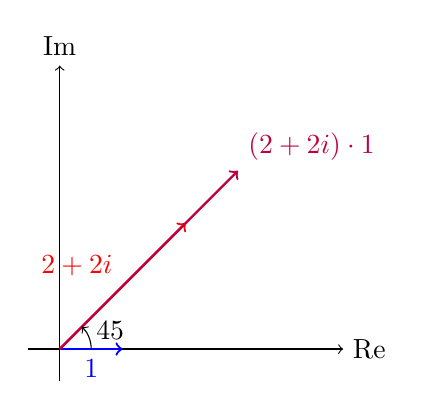
\begin{tikzpicture}[scale=0.8]
    \draw[->] (-0.5,0) -- (4.5,0) node[right] {Re};
    \draw[->] (0,-0.5) -- (0,4.5) node[above] {Im};
    \draw[->,thick,blue] (0,0) -- (1,0) node[midway,below] {$1$};
    \draw[->,thick,red] (0,0) -- (2,2) node[midway,above left] {$2+2i$};
    \draw[->,thick,purple] (0,0) -- (2.83,2.83) node[above right] {$(2+2i)\cdot 1$};
    \draw[->] (0.5,0) arc (0:45:0.5);
    \node at (0.8,0.3) {$45°$};
  \end{tikzpicture}
  \end{center}
  
  \textbf{Rotation de 45°} et \textbf{allongement} par un facteur $|2+2i| = 2\sqrt{2}$.
\end{frame}

\begin{frame}{Le module}
  Le \textbf{module} (ou norme) d'un nombre complexe mesure la longueur du vecteur $(x, y)$:
  \[
    |z| = \sqrt{x^2 + y^2}
  \]
  
  \begin{center}
  \begin{tikzpicture}[scale=1.2]
    \draw[->] (-0.5,0) -- (3.5,0) node[right] {Re};
    \draw[->] (0,-0.5) -- (0,2.5) node[above] {Im};
    \draw[->,thick,blue,line width=1.5pt] (0,0) -- (2.5,1.5) node[midway,above left] {$|z|$};
    \draw[dashed] (2.5,0) node[below] {$x$} -- (2.5,1.5);
    \draw[dashed] (0,1.5) node[left] {$y$} -- (2.5,1.5);
    \draw (0.5,0) arc (0:31:0.5);
    \node at (0.8,0.2) {$\theta$};
  \end{tikzpicture}
  \end{center}
\end{frame}

\begin{frame}{Interprétation trigonométrique}
  La trigonométrie nous permet d'interpréter $z = x + iy$ comme:
  \[
    z = |z| \left[ \cos(\theta) + i\sin(\theta) \right]
  \]
  
  où $\theta$ est l'angle que fait le vecteur avec l'axe réel.
  
  \bigskip
  Relations:
  \[
    x = |z| \cos(\theta) \qquad y = |z| \sin(\theta)
  \]
  \[
    |z| = \sqrt{x^2 + y^2} \qquad \theta = \arctan\left(\frac{y}{x}\right)
  \]
\end{frame}

\section{Complexe conjugué et division}

\begin{frame}{Division comme rotation inverse}
  
  Pour inverser une rotation d'angle $\theta$, on effectue une rotation d'angle $-\theta$.
  
  \bigskip
  Ceci nous amène au concept de \textbf{complexe conjugué}, noté $z^*$ (ou $\bar{z}$):
  \[
    z^* = x - iy
  \]
  
  En notation trigonométrique:
  \[
    z^* = |z|[\cos(-\theta) + i\sin(-\theta)] = |z|[\cos(\theta) - i\sin(\theta)]
  \]
  
\end{frame}

\begin{frame}{Le complexe conjugué}
  \begin{center}
  \begin{tikzpicture}[scale=1.2]
    \draw[->] (-0.5,0) -- (3.5,0) node[right] {Re};
    \draw[->] (0,-2,0) -- (0,2) node[above] {Im};
    \draw[->,thick,blue] (0,0) -- (2.5,1.5) node[midway,above left] {$z$};
    \draw[->,thick,red] (0,0) -- (2.5,-1.5) node[midway,below left] {$z^*$};
    \draw[dashed] (2.5,1.5) -- (2.5,-1.5);
    \draw (0.7,0) arc (0:31:0.7);
    \draw (0.7,0) arc (0:-31:0.7);
    \node at (1,0.3) {$\theta$};
    \node at (1,-0.3) {$-\theta$};
  \end{tikzpicture}
  \end{center}
  
  \[
    z \cdot z^* = (x + iy)(x - iy) = x^2 + y^2 = |z|^2
  \]
\end{frame}

\begin{frame}{Division de nombres complexes}
  Pour diviser par un nombre complexe, on multiplie par le conjugué divisé par le module au carré:
  \[
    \frac{1}{z} = \frac{z^*}{zz^*} = \frac{z^*}{|z|^2} = \frac{x - iy}{x^2 + y^2}
  \]
  
  \bigskip
  Pour diviser deux complexes:
  \[
    \frac{z_1}{z_2} = \frac{z_1 \cdot z_2^*}{|z_2|^2}
  \]
\end{frame}

\begin{frame}{Division détaillée en notation $x + iy$}
  Calculons $\frac{z_1}{z_2} = \frac{x_1 + iy_1}{x_2 + iy_2}$:
  
  \begin{align*}
    \frac{x_1 + iy_1}{x_2 + iy_2} &= \frac{(x_1 + iy_1)(x_2 - iy_2)}{(x_2 + iy_2)(x_2 - iy_2)} \\
    &= \frac{(x_1 x_2 + y_1 y_2) + i(y_1 x_2 - x_1 y_2)}{x_2^2 + y_2^2} \\
    &= \frac{x_1 x_2 + y_1 y_2}{x_2^2 + y_2^2} + i\frac{y_1 x_2 - x_1 y_2}{x_2^2 + y_2^2}
  \end{align*}
\end{frame}

\section{Représentation polaire}

\begin{frame}{Notation polaire}

  Notation $z = |z| e^{i\theta}$ qui sépare de manière élégante:
  
  \bigskip
  \begin{itemize}
    \setlength{\itemsep}{1em}
    \item Le \textbf{module} $|z|$: l'amplitude, la longueur
    \item La \textbf{phase} $\theta$: l'angle, la direction
  \end{itemize}

  \bigskip
  L'exponentielle transforme les multiplications en sommes sur les angles:
  \[
    z_1 \cdot z_2 = |z_1| e^{i\theta_1} \cdot |z_2| e^{i\theta_2} = |z_1||z_2| e^{i(\theta_1 + \theta_2)}
  \]

\end{frame}

\begin{frame}{Formule d'Euler}
  La \textbf{formule d'Euler} établit le lien entre l'exponentielle et les fonctions trigonométriques:
  \[
    e^{i\theta} = \cos(\theta) + i\sin(\theta)
  \]
  
  \bigskip
  Cas particuliers remarquables:
  \begin{align*}
    e^{i\pi/2} = i \qquad\qquad
    e^{i\pi} = -1 \qquad\qquad
    e^{2i\pi} = 1 \qquad\qquad
  \end{align*}
\end{frame}

\begin{frame}{Opérations en notation polaire}
  \textbf{Multiplication:}
  \[
    z_1 \cdot z_2 = (|z_1| e^{i\theta_1})(|z_2| e^{i\theta_2}) = |z_1||z_2| \, e^{i(\theta_1+\theta_2)}
  \]
  
  \textbf{Division:}
  \[
    \frac{z_1}{z_2} = \frac{|z_1| e^{i\theta_1}}{|z_2| e^{i\theta_2}} = \frac{|z_1|}{|z_2|} \, e^{i(\theta_1-\theta_2)}
  \]
  
  \textbf{Puissance:}
  \[
    z^n = (|z| e^{i\theta})^n = |z|^n e^{in\theta}
  \]
  
  \textbf{Racine n-ième:}
  \[
    \sqrt[n]{z} = |z|^{1/n} e^{i\theta/n}
  \]
\end{frame}

\begin{frame}{Racines de l'unité}
  Les racines n-ièmes de l'unité sont les solutions de $z^n = 1$:
  \[
    \omega_k = e^{2\pi i k/n} \qquad k = 0, 1, 2, \ldots, n-1
  \]
 
  \begin{center}
  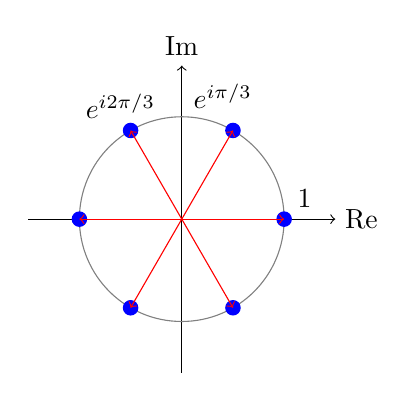
\begin{tikzpicture}[scale=1.3]
    \draw[->] (-1.5,0) -- (1.5,0) node[right] {Re};
    \draw[->] (0,-1.5) -- (0,1.5) node[above] {Im};
    \draw[gray] (0,0) circle (1);
    \foreach \k in {0,1,2,3,4,5} {
      \filldraw[blue] ({cos(60*\k)},{sin(60*\k)}) circle (2pt);
      \draw[->,red,thin] (0,0) -- ({cos(60*\k)},{sin(60*\k)});
    }
    \node at (1.2,0.2) {$1$};
    \node at (0.4,1.2) {$e^{i\pi/3}$};
    \node at (-0.6,1.1) {$e^{i2\pi/3}$};
  \end{tikzpicture}
  \end{center}
  \end{frame}

\section{Pour aller plus loin}

\begin{frame}{Vidéos par 3Blue1Brown} 
  \begin{center}
    \includegraphics[width=\linewidth]{../../figures/3b1b_complexes.png}
  \end{center}
\end{frame}

\begin{frame}{Quaternions et rotations 3D}
  Les quaternions étendent les nombres complexes pour les rotations 3D.
  
  \bigskip
  Nombres $1, i, j, k$ avec la table de multiplication:
  
  \begin{center}
  \begin{tabular}{c|cccc}
    $\times$ & $1$ & $i$ & $j$ & $k$ \\
    \hline
    $1$ & $1$ & $i$ & $j$ & $k$ \\
    $i$ & $i$ & $-1$ & $k$ & $-j$ \\
    $j$ & $j$ & $-k$ & $-1$ & $i$ \\
    $k$ & $k$ & $j$ & $-i$ & $-1$
  \end{tabular}
  \end{center}
  
  \bigskip
  Utilisés en graphisme 3D et jeux vidéo. En physique, on préfère les matrices de Pauli.

  \bigskip
  Ce petit exercice peut être continué avec des transformations plus générales que des rotations: cela amène à la \textbf{théorie des groupes} et de leurs représentations.
  
\end{frame}

\begin{frame}{Résumé}
  \begin{itemize}
    \setlength{\itemsep}{0.7em}
    \item Les complexes résolvent le problème de $\sqrt{-1}$
    \item Trois représentations: cartésienne, vectorielle, polaire
    \item La notation polaire $|z|e^{i\theta}$ sépare amplitude et phase (étirement et rotation)
  \end{itemize}
\end{frame}

\end{document}
